\chapter{Methods}

\begin{center}
    \textit{Here, the development process and methodologies are described in detail. This includes the design and implementation of the desktop application, the selection of tools and frameworks, and the approach to solving the problem.}
\end{center}

\section{Development Methodology}
\label{sec:development-methodology}

\subsection{Agile Approach}

\subsection{Sprint Planning}

\subsection{Code Reviews}

\section{Software Design}
\label{sec:software-design}

\subsection{Design Process}

\subsubsection*{User-Centered Design}

\subsection{Diagrams}

\subsubsection*{Sequence Diagram}

% \begin{figure}[h!]
%     \centering
%     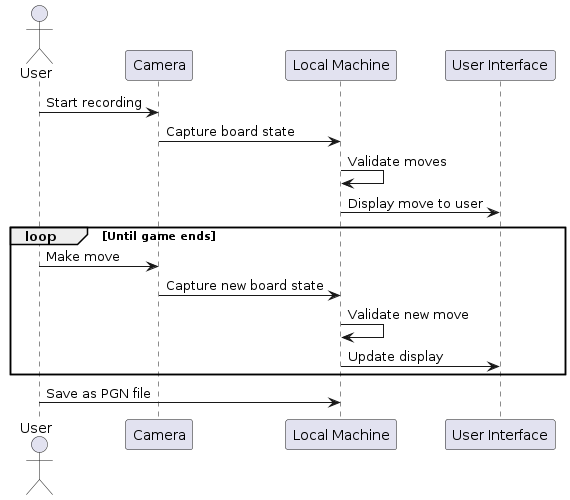
\includegraphics[width=0.75\linewidth]{figures/uml/sequence.png}
%     \caption[Sequence Diagram]{Sequence Diagram}
%     \label{fig:sequence}
% \end{figure}

\subsubsection*{Activity Diagram}

% \begin{figure}[h!]
%     \centering
%     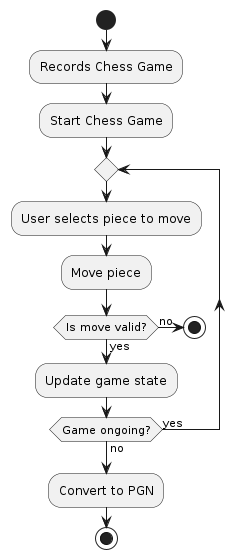
\includegraphics[height=0.75\linewidth]{figures/uml/activity.png}
%     \caption[Activity Diagram]{Activity Diagram}
%     \label{fig:activity}
% \end{figure}

\subsection{Wireframes}

\subsubsection*{Tournament Overview}

% \begin{figure}[h!]
%     \centering
%     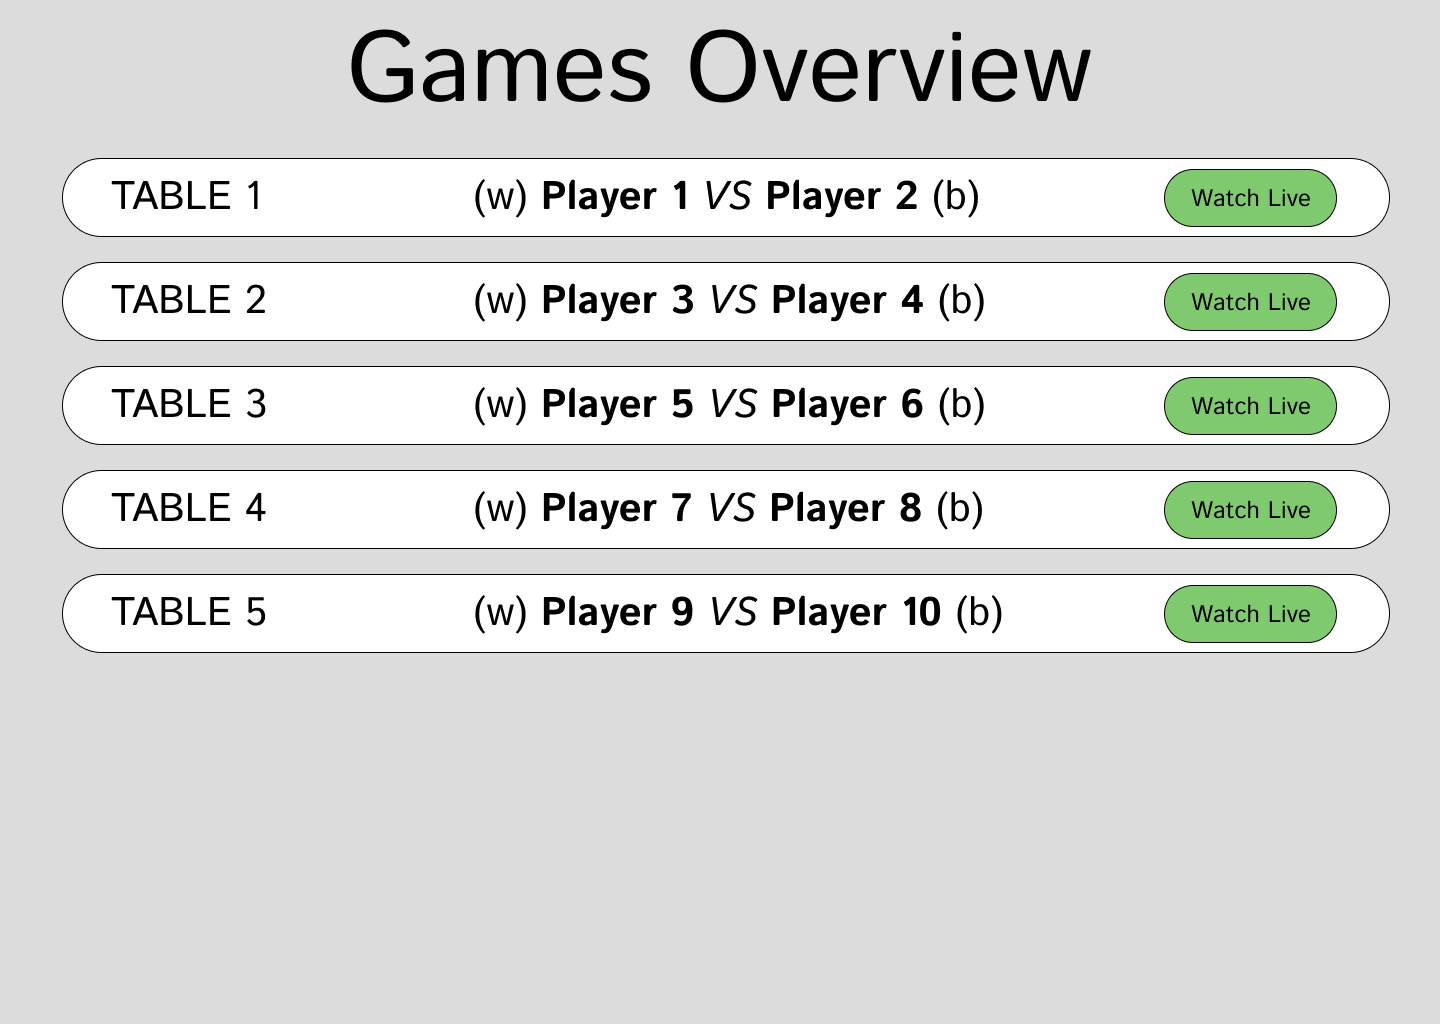
\includegraphics[width=0.75\linewidth]{figures/wireframe/overview.png}
%     \caption[Games Overview Wireframe]{Wireframe of the Games Overview}
%     \label{fig:app-overview}
% \end{figure}

\subsubsection*{Table View}

% \begin{figure}[h!]
%     \centering
%     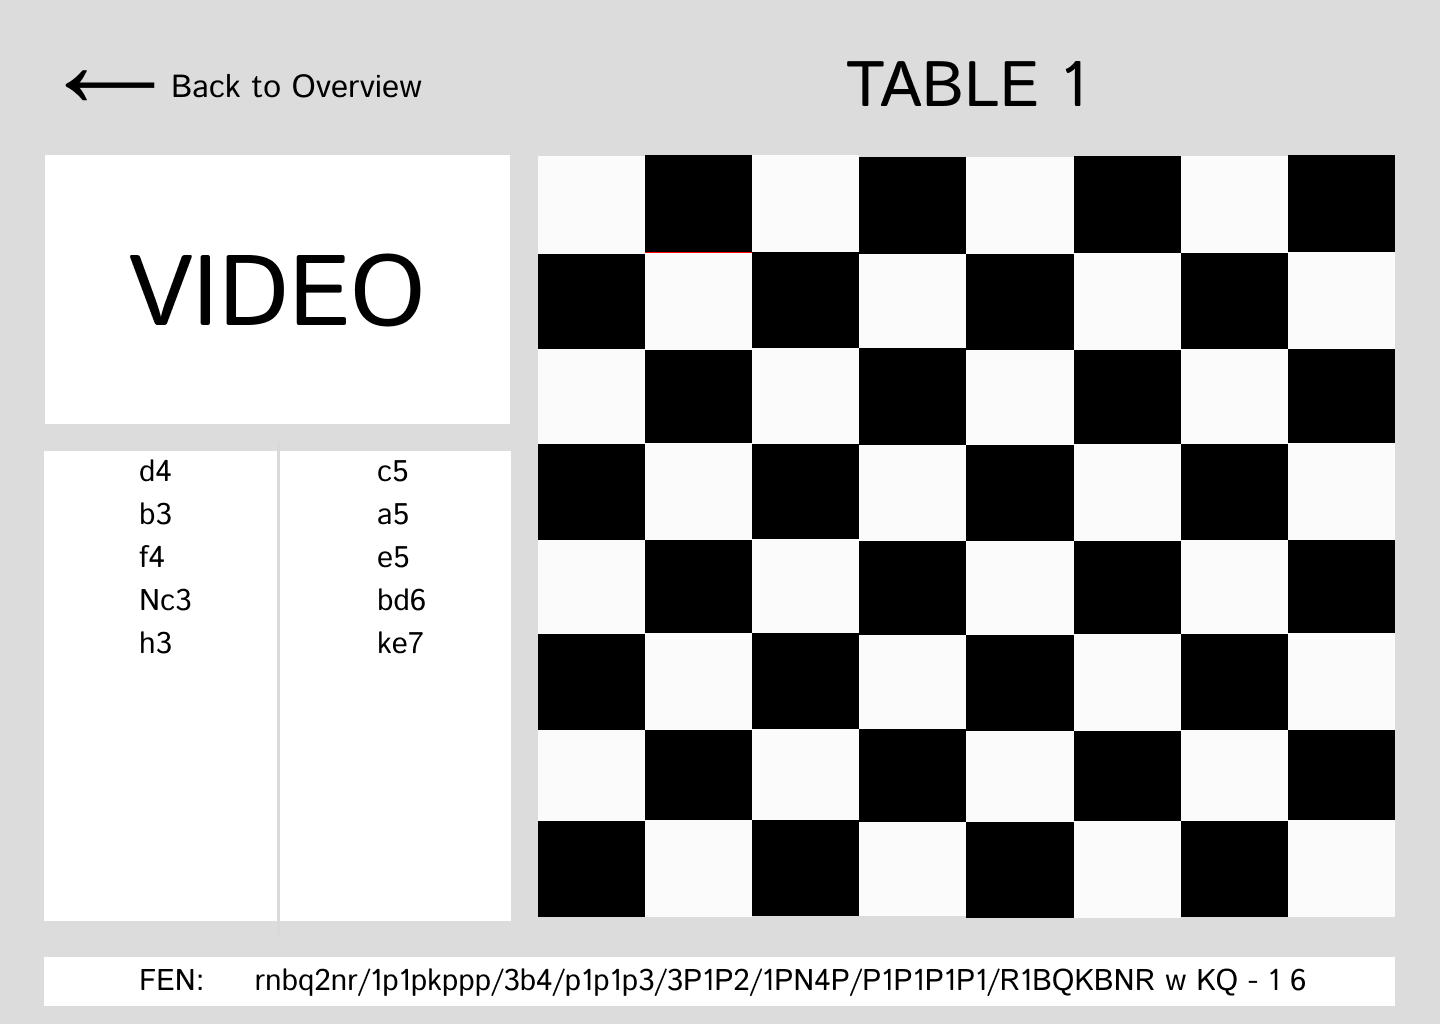
\includegraphics[width=0.75\linewidth]{figures/wireframe/table-view.png}
%     \caption[Table View Wireframe]{Wireframe of the Table View of a Game on Table 1}
%     \label{fig:app-table-view}
% \end{figure}

\section{Tools and Platforms}
\label{sec:tools}

\subsection{Development Tools}

\subsubsection*{Visual Studio Code}

\subsubsection*{Postman}

\subsubsection*{Netron.app}

\subsubsection*{Git}

\subsubsection*{ChatGPT}

\subsection{Collaboration and Design Tools}

\subsubsection*{GitHub}

\subsubsection*{Figma}

\subsubsection*{OneDrive}

\subsubsection*{Overleaf}

\section{Technology Stack}
\label{sec:tech-stack}

\subsection{Backend}
\subsubsection*{Python Libraries}

\begin{itemize}
    \item \texttt{chess} is a library for Python, with move generation, move validation, and support for common formats. \cite{python:chess}
    
    \item \texttt{FastAPI} is a modern and fast web framework for building \Glspl{api} with Python. \cite{python:fastapi}
    
    \item \texttt{numpy} is a fundamental package for scientific computing in Python. \cite{python:numpy}
    
    \item \texttt{onnxruntime}, \texttt{onnxruntime-gpu} assists in model serialization and interface with ORT. \cite{python:onnx}
    
    \item \texttt{opencv-python}, \texttt{opencv-contrib-python}, \texttt{opencv-python-headless} is used to solve computer vision problems. \cite{python:opencv}
    
    \item \texttt{requests} allows to send HTTP requests easily. \cite{python:requests}
    
    \item \texttt{scipy} is a fundamental package for algorithms for scientific computing in python. \cite{python:scipy}
    
    \item \texttt{tensorflow}, \texttt{tensorflow-intel} makes it easy to create ML models that can run in any environment. \cite{python:tensorflow}
\end{itemize}

\subsection{Frontend}
\subsubsection*{TypeScript Libraries}

\begin{itemize}
    \item \texttt{Vite} is a fast frontend build tool of web applications. \cite{ts:vite}
    
    \item \texttt{React} builds user interfaces out of individual pieces called components. \cite{ts:react}
    
    \item \texttt{@vitejs/plugin-react-swc} Speeds up the Vite development server. \cite{ts:swc}
    
    \item \texttt{chess.ts} a Typescript chess library for chess move generation/validation, piece placement/movement, and check/checkmate/draw detection \cite{ts:chess}
    
    \item \texttt{react-dom} serves as the entry point to the DOM and server renderers for React. \cite{ts:react-dom}
\end{itemize}